\documentclass{article}
\usepackage{tikz}

\begin{document}
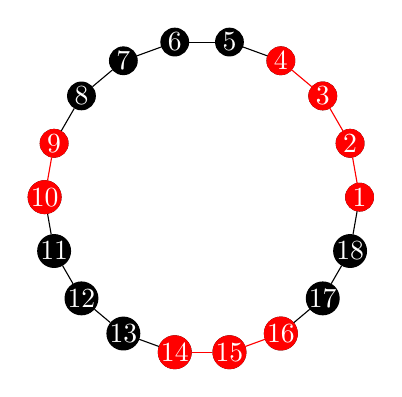
\begin{tikzpicture}
  \tikzstyle{every node}=[draw,circle,fill=black,minimum size=10pt,inner sep=0pt,text=white]
  \tikzstyle{selected}=[fill=red,draw=red]

  % Define the vertices
  \foreach \x in {1,...,18} {
    \node (\x) at ({360/18 * (\x - 1)}:2) {\x};
  }

  % Define the red vertices
  \foreach \vertex in {1,2,3,4,9,10,14,15,16} {
    \node[selected] at (\vertex) {\vertex};
  }

  % Draw the specified edges in red
  \foreach \a/\b in {1/2, 2/3, 3/4, 9/10, 14/15, 15/16} {
    \draw[selected] (\a) -- (\b);
  }

  % Draw the rest of the cycle edges in black
  \foreach \x/\y in {4/5, 5/6, 6/7, 7/8, 8/9, 10/11, 11/12, 12/13, 13/14, 16/17, 17/18, 18/1} {
    \ifnum\x=1\relax\else
    \draw (\x) -- (\y);
    \fi
  }
\end{tikzpicture}
\end{document}
